\documentclass[UTF8,9pt]{ctexart}
\usepackage{../../template/homeworkTEMP/hw}
\usepackage{listings}
\setcounter{secnumdepth}{0}
\usepackage{color}
\definecolor{dkgreen}{rgb}{0,0.6,0}
\definecolor{gray}{rgb}{0.5,0.5,0.5}
\definecolor{mauve}{rgb}{0.58,0,0.82}
\lstset{frame=tb,
        language=Python,
        aboveskip=3mm,
        belowskip=3mm,
        showstringspaces=false,
        columns=flexible,
        basicstyle={\small\ttfamily},
        numbers=none,
        numberstyle=\tiny\color{gray},
        keywordstyle=\color{blue},
        commentstyle=\color{dkgreen},
        stringstyle=\color{mauve},
        breaklines=true,
        breakatwhitespace=true,
        tabsize=3
}
\title{数值分析实验二} 
\begin{document} 
\maketitle
\se{1}
\sub{(1)}
先计算$\dis l(x,j) = \prod_{i=0,i\neq j}^k \f{x-x_i}{x_j-x_i}$, 再计算$\dis L(x)=\sum_{j=0}^k y_jl(x,j)$. 得到拉格朗日插值多项式, 然后分别在区间[-1,1], [0.9,1.0], [-1.1,-0.9]绘图 (如图1-3), 其中带$x$的线是真实的$f(x)$. 可以发现当$x$远离原点时, $L(x)$会迅速偏差远离$f(x)$. 同时随着$k$增大, 在$x=1$处的插值多项式的值会在$f(1)$上下震荡. $k=7$虽然是最高阶项, 但由于这种震荡在$x=1$处却误差最大. 同理在$x=-1$附近, 由于$x=-1$是节点因此没有误差, 但在稍小于或稍大于$x=-1$处均会有震荡现象出现. 
\begin{figure}[htbp]
        \centering
        \begin{minipage}[t]{0.48\textwidth}
        \centering
        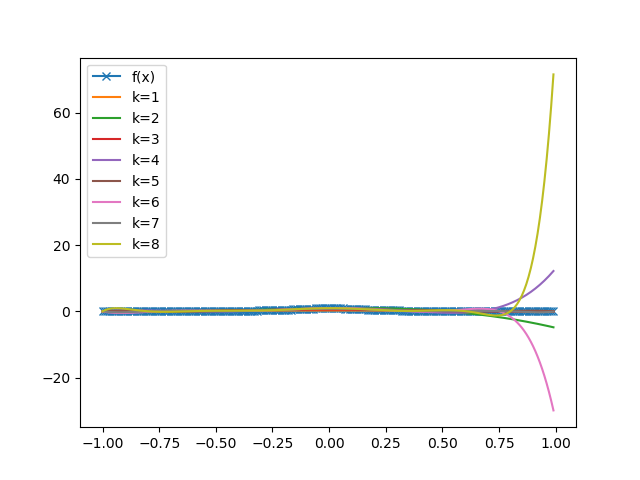
\includegraphics[scale=0.4]{1.png}
        \caption{[-1,1]区间内函数图像}
        \end{minipage}
        \begin{minipage}[t]{0.48\textwidth}
        \centering
        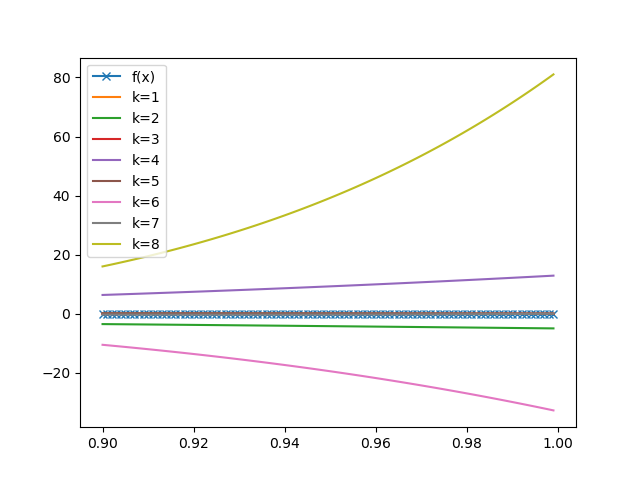
\includegraphics[scale=0.4]{2.png}
        \caption{[0.9,1]区间内函数图像}
        \end{minipage}
\end{figure}
\begin{figure}[htbp]
        \centering
        \begin{minipage}[t]{0.48\textwidth}
        \centering
        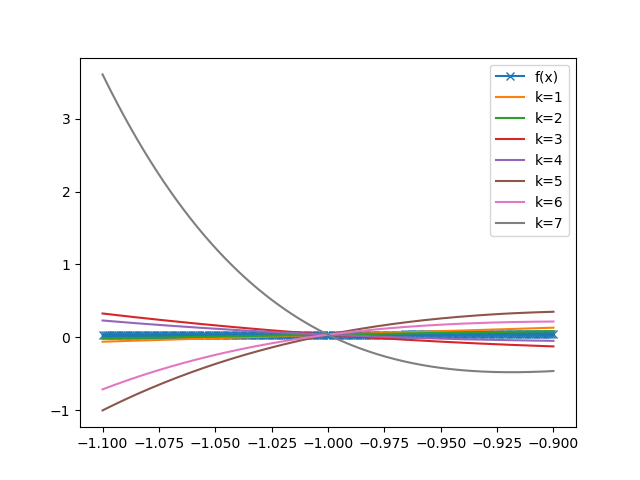
\includegraphics[scale=0.4]{3.png}
        \caption{[-1.1,-0.9]区间内函数图像}
        \end{minipage}
\end{figure}
\begin{figure}[htbp]
\begin{lstlisting}
        import numpy as np                    #第一题第一问
        import matplotlib.pyplot as plt       
        def f(x): return 1/(1+25*x**2)        #定义f(x)=1/(1+25x^2)
        def l(x,j,k,xs):                      #定义l(x)
            prod = 1                          
            for i in range(k+1):              #当i不等于j时, 乘以(x-xi)/(xj-xi)
                if i != j:prod *= (x-xs[i])/(xs[j]-xs[i])   
            return prod                       
        def L(x,k,xs,ys):                    #定义L(x)
            suml = 0                         #将所有l(x)相加
            for j in range(k+1): suml += ys[j]*l(x,j,k,xs)
            return suml
        x = np.arange(-1,1,0.01)             #定义域设为[-5,5]
        plt.plot(x,f(x),marker="x")          #绘制f(x)图像
        for k in range(2,7):                 #把k=2-6的几种情况绘图
            xs = np.arange(-1, 1, 2/(k+1))
            ys = f(xs)
            fig = plt.plot(x,L(x,k,xs,ys))
        plt.legend(labels = ['f(x)','k=1','k=2', 'k=3', 'k=4', 'k=5', 'k=6'])
        plt.show()
\end{lstlisting}
\end{figure}
\sub{(2)}
其法方程组为:
$$\left[ {\begin{array}{*{20}{c}}
	{(1, 1)}&{(x, 1)}&{(x^2, 1)}&{(x^3, 1)}&{(x^4 ,1)}\\
	{(1, x )}&{(x, x )}&{(x^2, x)}&{(x^3, x)}&{(x^4 , x)}\\
	{(1, x^2 )}&{(x, x^2 )}&{(x^2, x^2)}&{(x^3, x^2)}&{(x^4 , x^2)}\\
	{(1, x^3 )}&{(x, x^3 )}&{(x^3, x^3)}&{(x^3, x^3)}&{(x^4 , x^3)}\\
	{(1, x^4 )}&{(x, x^4 )}&{(x^4, x^4)}&{(x^4, x^4)}&{(x^4 , x^4)}
	\end{array}} \right]\left[ {\begin{array}{*{20}{c}}
	{{c_0}}\\
	{{c_1}}\\
	{{c_2}}\\
	{{c_3}}\\
	{{c_4}}
	\end{array}} \right] = \left[ {\begin{array}{*{20}{c}}
	{(f,1)}\\
	{(f,x )}\\
	{(f,x^2 )}\\
	{(f,x^3 )}\\
	{(f,x^4 )}
	\end{array}} \right]$$
其中内积的定义为$(f,g)=\int_{-1}^1 f(x)g(x)\d x$, 计算出左方关于$x$的矩阵$X$和右边$f$与不同阶数的$x$的乘积的矩阵$B$便可算出系数矩阵$C$, 该矩阵即为$P(x)$中各阶$x$的系数矩阵. 计算可得:
$$P_4(x) =  0.6694-2.3055 x^2+1.8689 x^4$$
绘制$f(x)$和$P(x)$如图4所示: 
\begin{figure}[htbp]
	\centering
	\begin{minipage}[t]{0.48\textwidth}
	\centering
	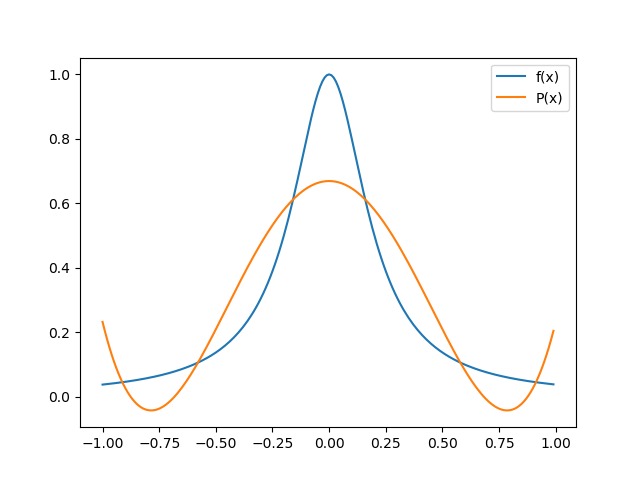
\includegraphics[scale=0.4]{4.png}
	\caption{[-1,1]区间内函数图像}
	\end{minipage}
\end{figure}
\begin{figure}[htbp]
	\begin{lstlisting}
		import numpy as np                  #第一题第二问
		import sympy
		import matplotlib.pyplot as plt
		x,X,B = sympy.symbols('x'),np.empty([5,5]),np.empty([5,1])
		def innerprod(x,f,g): return sympy.integrate(f*g,(x,-1,1))#定义两函数内积为二者乘积在[-1,1]的积分
		for i in range(5):                 #分别为法方程中的两个矩阵X,B赋值
			for j in range(5): X[i][j] = innerprod(x,x**i,x**j) 
			B[i] = innerprod(x,1/(1+25*x**2),x**i)
		C = np.matmul(np.mat(X).I,B).flat  #求解系数矩阵C=X^-1B
		print(C)                           #C = [0.67,0,-2.3,0,1.87] 可以看到x,x^3项系数均为0.
		x = np.arange(-1,1,0.01)           #定义绘图定义域为[-1,1]
		P = C[0]+C[2]*x**2+C[4]*x**4       #计算定义域内P(x)
		plt.plot(x,1/(1+25*x**2))          #绘制f(x)图像
		plt.plot(x,P)                      #绘制P(x)图像
		plt.legend(labels = ['f(x)','P(x)'])
		plt.show()
	\end{lstlisting}
\end{figure}
\sub{(3)}
	设$I=\int_{-1}^{1}\left[f(x)-P_{4}(x)\right]^{2} \mathrm{d} x$, 复合辛普森公式为$$ 
\begin{array}{c}{S= \frac{2}{6 n}\left\{g(-1)+4\left[g\left(x_{1}\right)+g\left(x_{3}\right)+\cdots+g\left(x_{2 n-1}\right)\right]\right.} \\ {+2\left[g\left(x_{2}\right)+g\left(x_{4}\right)+\dots+g\left(x_{2 n-2}\right)\right]+g(1) \}}\end{array}
 $$
取$n=100$, 计算可得$S = 0.18349$. 即为其均方差. 
\begin{figure}[htbp]
	\begin{lstlisting}
		import numpy as np            ##第一题第三问, 定义两函数之差的平方为g(x)
		def g(x): return (1/(1+25*(x**2)) - (0.6694-2.3055*x**2+1.8689*x**4))**2  
		n = 100                       #在复合辛普森公式中取100个点
		xs = np.arange(-1,1,2/(2*n))
		S=(2/(6*n))*(g(-1)+4*sum([g(xs[2*i-1]) for i in range(1,n+1)])+2*sum([g(xs[2*i]) for i in range(1,n)])+g(1))  #计算S 
		print(np.sqrt(S))             #sqrt(S) = 0.18349445771001033
	\end{lstlisting}
\end{figure}
\se{2}
所要求解的超定方程组的矩阵形式为:
$$\left(\ar{1&t_1\\2&t_2\\\vdots&\vdots\\9&t_9}\right)\left(\ar{a\\b}\right) = \left(\ar{y_1\\y_2\\\vdots\\y_9}\right)$$
设其为$Ax=b$, 则$x=(A^TA)^{-1}A^Tb$可求得$x$并求得$a=-33.03828,b=0.01859$. 再代入模型$N(t)=e^{a+b t}$可得到$N(2018)=88.4, N(2019)=90.0$亿. 
\begin{figure}[htbp]
	\begin{lstlisting}
		import numpy as np #第二题
		A = np.mat(np.c_[np.ones(9), np.arange(1960, 1969)])
		y = np.log([29.72, 30.61, 31.51, 32.13, 32.34, 32.85, 33.56, 34.2, 34.83])
		a, b = np.matmul(np.matmul(np.matmul(A.T, A).I, A.T), y).flat
		print(a, b, np.exp(a+b*2018), np.exp(a+b*2019))		
	\end{lstlisting}
\end{figure}
\se{3}
共有九组数据, 取4月20日为疫情爆发第一天$x=1$. 所要求解的超定方程组的矩阵形式为:
$$\left(\ar{1&1/x_1\\2&1/x_2\\\vdots&\vdots\\9&1/x_9}\right)\left(\ar{a\\b}\right) = \left(\ar{1/y_1\\1/y_2\\\vdots\\1/y_9}\right)$$
利用与上题相同的方法, 可得6月25日(第67天)病人数量为2469人. 其中式中$a=0.0003659,b=0.00300659$.
\begin{figure}[htbp]
	\begin{lstlisting}
		import numpy as np
		x = np.array([1,11,12,21,31,41,43,52,62])
		A = np.mat(np.c_[np.ones(9), 1/x])
		y = np.array([297,1584,1640,1988,2189,2309,2309,2394,2439])
		a, b = np.matmul(np.matmul(np.matmul(A.T, A).I, A.T), 1/y).flat
		print(a, b, 1/(a+b/67))			
	\end{lstlisting}
\end{figure}
\end{document}